
% --------------- 12 POINT FONT -------------------------------
\documentclass[12pt]{article}
% --------------- 10 POINT FONT FOR CAPTIONS ------------------
\usepackage[font=footnotesize]{caption}
% --------------- NY TIMES FONT -------------------------------
\usepackage{times}
% --------------- 1 INCH MARGINS ------------------------------
\usepackage[margin=1in]{geometry}
% --------------- LINE SPACING --------------------------------
\usepackage{setspace}
\singlespacing
%\doublespacing
% --------------- SMALL SECTION TITLES ------------------------
\usepackage[tiny,compact]{titlesec}
% --------------- PACKAGES ------------------------------------
\usepackage{bookmark}
\usepackage{algorithm}
\usepackage{algpseudocode}
\usepackage{amsfonts}
\usepackage{amsmath}
\usepackage{amssymb}
\usepackage{amsthm}
\usepackage{bm}
\usepackage{color}
\usepackage{comment}
\usepackage{float}
\usepackage{graphicx}
%\usepackage[hidelinks]{hyperref}
\usepackage{makecell}
\usepackage[caption=false,font=footnotesize,subrefformat=parens,labelformat=parens]{subfig}
\usepackage{wrapfig}
\usepackage{url}
\usepackage[table]{xcolor}
\graphicspath{{images/}}
\begin{document}
% --------------- TITLE AND NAME ------------------------------
\begin{center}
\textbf{Summary}\\
\end{center}

\noindent
Bardia Mojra\\
\today\\
Seminar on Active Learning\\
Robotic Vision Lab\\
% --------------- CONTENT -------------------------------------
\begin{center}
{\large Task-Aware Variational Adversarial Active Learning\\}
% \end{center}
% \begin{center}
  {\small Kwanyoung Kim, Dongwon Park, Kwang In Kim, Se Young Chun}\\
  {\small CVPR 2021}\\
\end{center}

% \noindent
% \textbf{Introduction}
Deep learning requires large amounts of data to train properly and the high
cost of
labeling entire datasets have created an urgent need for more efficient
learning algorithms. \textit{Active learning (AL) aims to improve learning by
querying the most informative samples to be annotated unlabeled pool}.
Existing AL methods can be categorized into two main groups,
\textit{task-agnostic} and \textit{task-aware}. In this paper, the authors
propose a novel method that combines the two approaches and is able to achieve
state-of-the-art performance on multiple classification benchmarks.\\

Task-agnostic (or distribution-based) methods rely on distribution of labeled
or input data, \(P(x)\) to identify \textit{influential data points}. Such techniques
query samples in high-density regions and are good for learning the distribution of
standalone clusters but they do not make any determination on input-output
dependency. This becomes particularly important in classification
tasks where there is always the possibility of partial distribution overlap
among latent space variables from different classes.\\

Task-aware (or model uncertainty-based) methods address this limitation by
modeling such dependence,
e.g. via estimating the conditional distribution \(P(y|x)\). Such methods
identify \textit{difficult data points} by querying samples from high uncertainty
regions, e.g. overlapping or boundary regions.
Task-agnostic methods do not exploit structures from tasks and task-aware
methods do not seem to well-utilize overall data distribution. Recently,
SRAAL introduced a method that combines task-aware and
task-agnostic approached with an uncertainty indicator and with a unified
representation for both labeled and unlabeled data \cite{SRAAL}.
Even though SRAAL achieved state-of-the-art performance, it did not use
information directly about the task \cite{LearningLoss} and its learner
seems to be limited to only VAE-type networks with a latent space for its
unified representation.\\

In this paper, the authors propose a novel method which builds upon
variational adversarial active learning \cite{VAAL} and utilizes
\cite{LearningLoss} to exploit the structure \(P(y|x)\) of the problem at hand.
Moreover, the authors, 1) propose to relax the goal of loss prediction module from
accurate loss prediction to loss ranking prediction \cite{RankCGAN}. 2) Introduce
\textit{Task-Aware Variational Adversarial Active Learning} (TA-VAAL) to embed
the normalized ranking loss information from any given task learner (with or
without latent state representation). 3) Demonstrate state-of-the-art
performance over Learning Loss \cite{LearningLoss}, VAAL \cite{VAAL}, Coreset
\cite{coreset}, Monte-Carlo dropout \cite{MonteCarloDropout} on CIFAR10, CIFAR100,
Caltech101, imbalanced CIFAR10, and on Cityscapes semantic segmentation
benchmark dataset.\\

\noindent
\textbf{Learning Loss Ranker}
Based on \cite{LearningLoss}, it trains to predict relative rankings
of losses instead of predicting the actual losses. The loss rankings are
then embedded into the latent space of VAAL with the conditional latent
variable r. Moreover, the ranker estimator is a smooth differentiable function
with nice convergence properties for optimization.

% \noindent
% \textbf{The figure}
\begin{figure}[h]
  \centering
  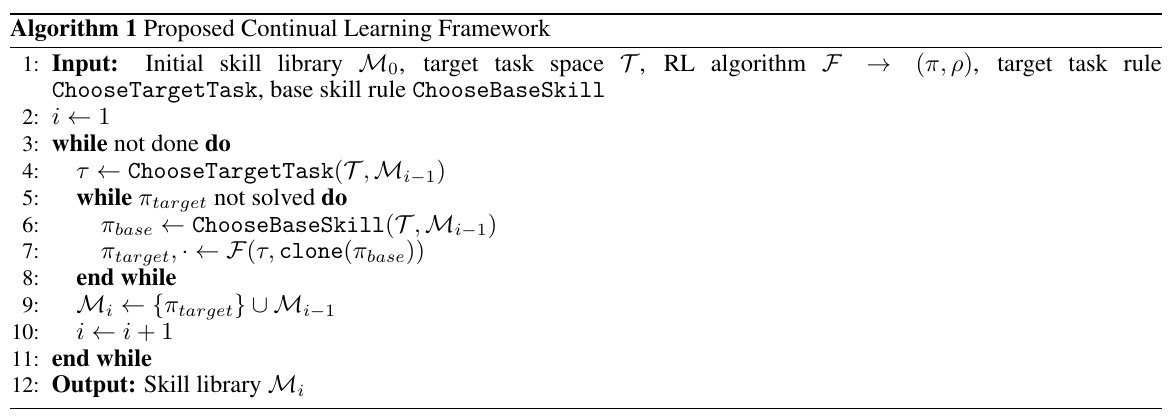
\includegraphics[width=1\textwidth]{/fig01.png}
  \caption{}
\end{figure}

\begin{figure}[h]
  \centering
  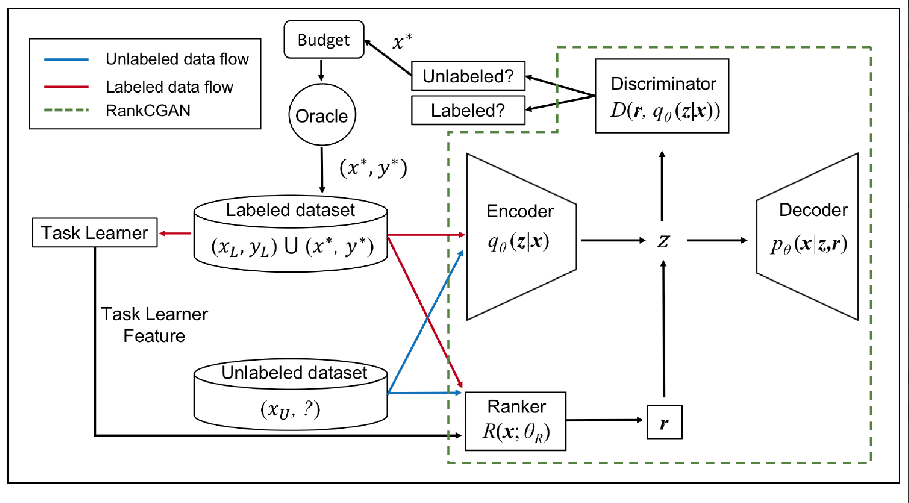
\includegraphics[width=.8\textwidth]{/fig02.png}
  \caption{TA-VAAL}
\end{figure}




%Sets the bibliography style to UNSRT and import the
\newpage

\bibliography{ref}
\bibliographystyle{ieeetr}

\end{document}
